%Einfache Vorlage f�r eine mit Latex realisierte Hausarbeit von http://www.studieren-info.de
%Du kannst diese Vorlage f�r deine Hausarbeit beliebig anpassen%


%-------------------
%Beginn des Kopfbereiches
%-------------------

%Wir verwenden eine DIN-A4-Seite und die Schriftgr��e 12.
\documentclass[a4paper,12pt,fontsize=12,DIV=12]{scrartcl} 


%Diese drei Pakete ben�tigen wir f�r die Umlaute, Deutsche Silbentrennung etc.
%Apple-Nutzer sollten anstelle von \usepackage[latin1]{inputenc} das Paket \usepackage[applemac]{inputenc} verwenden
\usepackage[utf8]{inputenc}
\usepackage[ngerman]{babel}
\usepackage[T1]{fontenc}
\usepackage{graphicx}
\usepackage{subfigure}
\usepackage[format=hang,justification=centering,singlelinecheck=off]{caption}

%Das Paket erzeugt ein anklickbares Verzeichnis in der PDF-Datei.
\usepackage{hyperref}

%Das Paket wird für die anderthalb-zeiligen Zeilenabstand benötigt
\usepackage{setspace}

%Einrückung eines neuen Absatzes
\setlength{\parindent}{0em}

%Definition der Ränder
\usepackage[paper=a4paper,left=30mm,right=30mm,top=30mm,bottom=30mm]{geometry} 

%Abstand der Fußnoten
\deffootnote{1em}{1em}{\textsuperscript{\thefootnotemark\ }}

%Regeln, bis zu welcher Tiefe (section,subsection,subsubsection) Überschriften angezeigt werden sollen (Anzeige der Überschriften im Verzeichnis / Anzeige der Nummerierung)
\setcounter{tocdepth}{3}
\setcounter{secnumdepth}{3}

%-------------------
%Ende des Kopfbereiches
%-------------------


%-------------------
%Hier beginnt der Text deiner Hausarbeit
%-------------------
\begin{document}


%Beginn der Titelseite
\begin{titlepage}
\begin{small}
\vfill {Universitaet Rostock\\ 
IEF/Institut für Automatisierungstechnik\\ 
Sommersemester 2012}
\end{small}


\begin{center}
\begin{Large}
\vfill {\textsf{\textbf{
	Hausarbeit - Hall-Software für das EZ-Kit BF533
}}}
\end{Large}
\end{center}

\begin{center}
\vspace{2.0cm}

\includegraphics[scale=0.8]{Bilder/Versuchsaufbau_Demonstration.png}
\end{center}

\begin{small}
\vfill Florian Grützmacher \\ Max-Planck-Str. 2a \\  18057 Rostock \\  florian.gruetzmacher@uni-rostock.de\\ 
\end{small}

\vspace{-5.0cm}

\begin{small}
\vfill Simeon Wiedenmann \\ Kiebitzberg 4 \\  18057 Rostock \\  simeon.wiedenmann@uni-rostock.de\\ 
\newline
\today
\end{small}

\end{titlepage}
%Ende der Titelseite


%Inhaltsverzeichnis (aktualisiert sich erst nach dem zweiten Setzen)
\tableofcontents
\thispagestyle{empty}

%Beginn einer neuen Seite
\clearpage

%Anderthalbzeiliger Zeilenabstand ab hier
\onehalfspacing

\pagestyle{plain}


\section{Einleitung}
Im Rahmen der Veranstaltungsreihe "`Signalprozessortechnik"' am Institut für Automatisierungstechnik der Universität Rostock wurden Kenntnisse über Funktionen und Leistungsfähigkeit verschiedener Signalprozessoren für den Einsatz digitaler Signalverarbeitung vermittelt.\footnote{siehe Vorlesungsverzeichnis der Universität Rostock, Veranstaltungsnr. 24141 }
Die Veranstaltung wurde im Sommersemester 2012 durch die Fakultät für Informatik und Elektrotechnik (IEF) der Universität Rostock angeboten und von Herrn Dr.-Ing. Wolf-Dieter Heinitz gehalten.
Neben den behandelten Schwerpunkten

 %Eine einfache Liste
 \begin{itemize} 
\item Digitale Signalverarbeitung: Vorteile, Probleme, Applikationen
\item Basisalgorithmen der digitalen Signalverarbeitung
\item Datenformate für die digitale Signalverarbeitung
\item Signalverarbeitung mit klassischen Mikrokontrollern
\item Universelle Signalprozessoren: Festkomma-Prozessor DSP 5630x, Gleitkomma-Prozessor TMS 320C3x, TMS320C4x
\item Übersicht zu anderen modernen Signalprozessoren und aktuellen Weiterentwicklungen Texas Instruments: C80, C62x, C67x, Analoge Devices: ADSP-21160, BF53x
\item Entwicklungswerkzeuge für DSP-Programmierung
\end{itemize}

galt es ein Abschlussprojekt zu Implementieren, es den Modulteilnehmern vorzustellen und das Vorgehen in einer Hausarbeit zu dokumentieren.

\section{Aufgabenstellung}

\subsection{Hall-Software für das EZ-Kit BF533}
Programmierung einer Software zur Erzeugung von künstlichem Hall. Ein analoges Eingangssignal von einem Mikrophon ist mit künstlichem Hall zu versehen und an einem analogen Ausgangskanal an einen Kopfhörer auszugeben.
\newline
Die Projektarbeit ist im Rahmen einer Demonstration an einem Testaufbau mit Mikrophon und Kopfhörer vorzuführen.

\subsection{Versuchsaufbau}
Bei der Implementation des künstlichen Halls ist es hilfreich, zunächst das Übertragungsverhalten des Digitalen Signalprozessors (DSP) beobachten zu können. Dazu wurde ein Versuchsaufbau für die Implementation eingerichtet, welcher hier zu sehen ist:
\begin{center}
%\vspace{2.0cm}
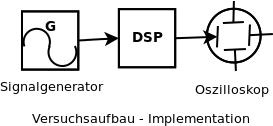
\includegraphics[scale=0.8]{Bilder/Versuchsaufbau_Implementation.png}
\end{center}
Ein am Signalgenerator erzeugtes Wunsch-Signal kann hierbei im DSP bearbeitet werden und das modifizierte Signal kann am Oszilloskop beobachtet werden.

Zur Demonstration des mit dem DSP erzeugten künstlichen Halls wird für bessere Anschaulichkeit jedoch folgender Versuchsaufbau genutzt.
\begin{center}
	%\vspace{2.0cm}
	
\includegraphics[scale=0.8]{Bilder/Versuchsaufbau_Demonstration.png}
\end{center}
%
%\begin{figure}
%	
\includegraphics[scale=0.8]{Bilder/Versuchsaufbau_Demonstration.png}
%	\caption{Titel der Grafik}
%	\label{labelname}
%\end{figure}
%
Ein Mikrofon wird an den Eingang des DSP angeschlossen und liefert ein analoges Eingangssignal. Dieses wird mit Hilfe eines Analog-Digital-Wandlers (ADC) digitalisisert und im DSP bearbeitet. Das digital bearbeitete Signal wird über einen Digital-Analog-Wandler DAC in ein analoges Ausgangssignal gewandelt, welches an den Lautsprechern ausgegeben wird.


\section{Digitale Signalverarbeitung}
Die Digitale Signalverarbeitung als Teilgebiet der Nachrichtentechnik beschäftigt sich mit der Verarbeitung digitaler Signale unter Einsatz von digitalen Systemen, wie z.B. Digitale Signalprozessoren.
Da unsere physikalische Umwelt jedoch häufig Analoge Signale als Eingangssignale (wie z.B. das Schwingen einer Membran im Mikrofon) sowie analoge Ausgangssignale (z.B. schwingende Lautsprechermembranen) verursacht, schließt die digitale Signalverarbeitung häufig auch eine Analog-Digital Wandlung des Eingangssignals und eine Digital-Analog Wandlung des Ausgangssignals mit ein.

\subsection{Das Prinzip digitaler Signalverarbeitung}
Um ein zeit-kontinuierliches und werte-kontinuierliches analoges Signal zu digitalisieren, muss es mit einer Abtastfrequenz $f_a$ abgetastet werden und auf einen quantisierten Wertebereich abgebildet werden. 
Um eine "`exakte"' Signalrekonstruktion sicherzustellen, muss das Nyquist-Shannon-Abtasttheorem eingehalten werden. Dieses besagt, dass die Abtastfrequenz $f_a$ mindestens so groß sein muss wie das doppelte der höchsten im Signal vorkommenden Frequenz $f_g$.
\begin{center}
\fbox{$f_a >= 2*f_g$} \footnote{Abtasttheorem }\\
\end{center}
Um dies sicherzustellen wird das analoge Eingangssignal x(t) mittels eines analogen Tiefpasses (TP) bandbegrenzt. Das abgetastete Signal ist bereits zeit-diskret.
%
\begin{figure}[h]
	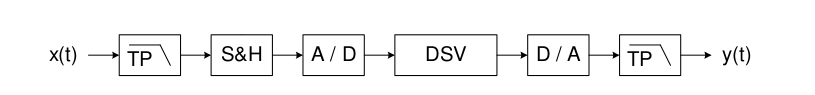
\includegraphics[scale=0.5]{Bilder/DSV_Blockschaltbild.png}
	\caption{Titel der Grafik}
	\label{labelname}
\end{figure}
%

%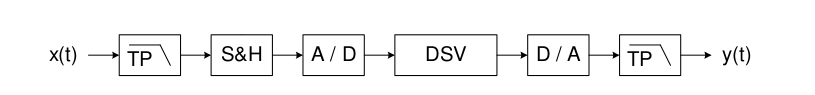
\includegraphics[scale=0.5]{Bilder/DSV_Blockschaltbild.png}


Ein Sampe and Hold Glied (S\&H) stellt sicher, dass der am Analog-Digital Wandler (A/D) anliegende Spannungswert für die Zeit eines Wandelvorgangs konstant gehalten wird.
Im Anschluss an die A/D Wandlung liegt ein zeit- und werte-diskretes Signal vor. Dieses digitale Signal kann nun mittels Digitaler Signalverarbeitung (DSV) wie gewünscht manipuliert werden. Dazu werden häuftig digitale Signalprozessoren eingesetzt.

Das digitale Signal muss nach der Verarbeitung erneut in ein analoges Signal gewandelt werden. Dies geschieht mithilfe des Digital-Analog Wandlers (D/A). Anschließend wird das Ausgangssignal noch durch einen analogen Rekonstruktions-Tiefpass (T/P) geglättet. Das so entstehende Ausgangssignal ist nun wieder analog und geht aus dem Eingangssignal x(t) durch digitale Signalverarbeitung hervor.

\subsection{Warum Signalprozessoren?}
Zzril delenit augue duis dolore te feugait nulla facilisi nam liber tempor. Nihil imperdiet doming; id quod mazim placerat facer possim assum? Mirum est notare quam littera gothica 
quam nunc putamus! Consectetuer adipiscing elit sed diam nonummy nibh euismod.

\section{Das Kit EZ-Kit BF533}
Dolore te feugait nulla facilisi nam liber tempor cum soluta nobis eleifend option. Amet consectetuer adipiscing elit sed diam nonummy nibh euismod tincidunt ut laoreet. In iis qui facit eorum; claritatem Investigationes demonstraverunt lectores legere me. In vulputate velit esse molestie consequat vel illum dolore. Wisi enim ad minim, veniam quis nostrud exerci. Facer possim assum typi non habent claritatem insitam est usus legentis lius quod.

Dolore te feugait nulla facilisi nam liber tempor cum soluta nobis eleifend option. Amet consectetuer adipiscing elit sed diam nonummy nibh euismod tincidunt ut laoreet. In iis qui facit eorum; claritatem Investigationes demonstraverunt lectores legere me. In vulputate velit esse molestie consequat vel illum dolore. Wisi enim ad minim, veniam quis nostrud exerci. Facer possim assum typi non habent claritatem insitam est usus legentis lius quod.

\section{Lösungsstrategie}
Dolore te feugait nulla facilisi nam liber tempor cum soluta nobis eleifend option. Amet consectetuer adipiscing elit sed diam nonummy nibh euismod tincidunt ut laoreet. In iis qui facit eorum; claritatem Investigationes demonstraverunt lectores legere me. In vulputate velit esse molestie consequat vel illum dolore. Wisi enim ad minim, veniam quis nostrud exerci. Facer possim assum typi non habent claritatem insitam est usus legentis lius quod.

Dolore te feugait nulla facilisi nam liber tempor cum soluta nobis eleifend option. Amet consectetuer adipiscing elit sed diam nonummy nibh euismod tincidunt ut laoreet. In iis qui facit eorum; claritatem Investigationes demonstraverunt lectores legere me. In vulputate velit esse molestie consequat vel illum dolore. Wisi enim ad minim, veniam quis nostrud exerci. Facer possim assum typi non habent claritatem insitam est usus legentis lius quod.

\subsubsection{Hall}
Hall bzw. Nachhall ist ein Effekt kontinuierlicher Reflexionen einer Schallwelle.
Wird eine Schallwelle an unterschiedlichen Stellen Reflektiert, und die Reflektierten Wellen, haben unterschiedliche laufzeiten aufgrund der unterschiedlichen Abstände zu den reflektierenden Objekten, treffen mehrere Reflektierte Schallwellen, der selben Ursprungs-Schallwelle mit unterschiedlichen Verzögerungszeiten aufeinander. Da der Schalldruck einer Schallwelle mit zunehmender Ausbreitungszeit aufgrund Luftreibung und mit zunehmender Anzahl an Reflektionen aufgrund von Wärmeverlusten abnimmt, sind reflektierte Schallwellen umso schwächer, je länger der Zeitpunkt ihrer Enstehung zurückliegt.
Hall wird unterteilt in frühe Reflektionen, welche 1-2 Reflektionen des Ursprungssignals sind, und diffusem Nachhall, welcher aus vielen Reflektionen mit stärkerer Abschwächung des Ursprungssignals besteht. Verantwortlich für den 'räumlichen' klang des Halls, sind die frühen Reflektionen, wobei der Nachhall wiederum aus Reflektionen der frühen Reflektionen entsteht und für mehr 'Volumen' sorgt.


\begin{figure}[h]
	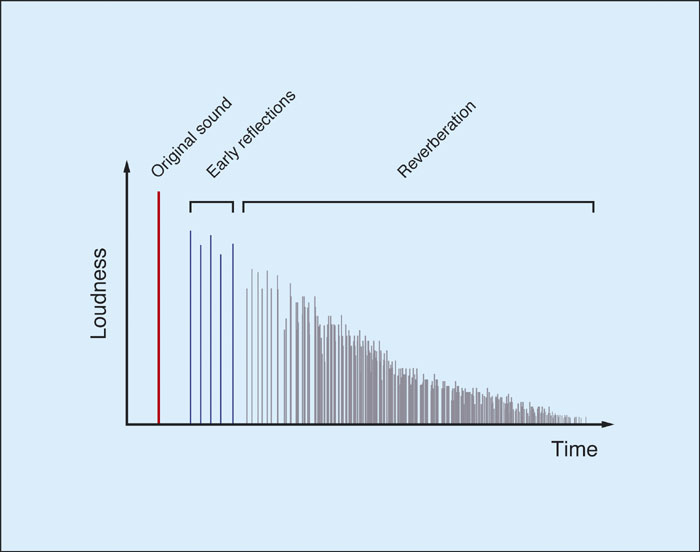
\includegraphics[scale=0.5]{Bilder/raumimpulsantwort.jpg}
	\caption{Raumimpulsantwort}
	\label{labelname}
\end{figure}
Quelle: http://www.offsetguitars.com/forums/viewtopic.php?f=11\&t=43975\&start=15

\subsubsection{Künstlicher Hall mit Infinite Impulse Response Filter}
Um mit dem DSP künstlichen Hall zu erzeugen, müssen die vom AD-Wandler erhaltenen Werte in einem Buffer gespeichert werden um zu einem späteren Zeitpunkt (50 bis 100 ms) darauf zurückgreifen zu können. Jeder neu abgetastete Wert wird mit einem Vorfaktor versehen und mit weiter zurückliegenden Signalwerten, ebenfalls mit bestimmtem Vorfaktoren akkumuliert und an den DA-Wandler übergeben. Zusätlich wird der akkumulierte Wert wieder mit einem Vorfaktor auf den nächsten neuen Wert aufaddiert. Durch die Akkumulation werden die frühen Reflektionen, durch die Rückkopplung der Nachhall simuliert. 
Die entspricht der Struktur eines IIR-Filters.
\begin{figure}[h]
	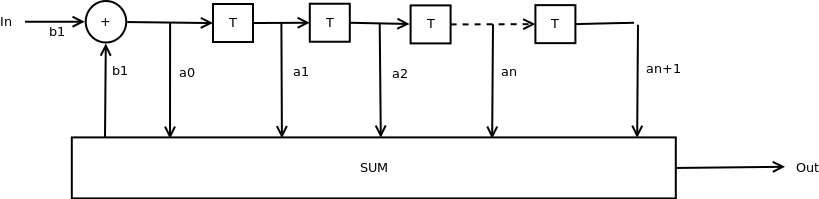
\includegraphics[scale=0.5]{Bilder/iir.png}
	\caption{IIR-Filter Struktur}
	\label{labelname}
\end{figure}

\subsubsection{Implementierung}
Um eine IIR-Struktur zu implementieren, haben wir einen Buffer(Array) mit 4096 Werten im fractional-32 Format deklariert. Für den Buffer und den Akkumulator wurden Fractional-32 Formate benutzt, da Multiplikationen von Fractional-16 Werten, ein Fractional-32 liefern und so ohne Schieben damit weitergerechnet werden kann.
Sobald am AD-Wandler ein neuer Wert anliegt, wird die Prozess-Funktion, im folgenden Prozess genannt, aufgerufen. Im Prozess wird der neue Wert zunächst gespeichert und mit einem dem Vorfaktor 0.5 im Buffer abgelegt. der Vorfaktor wird durch ein Right-Shift realisiert, was einer Division durch 2 entspricht.
Dieser Wert wird im Buffer abgelegt. Um das Verschieben von 4096 Werten pro Prozessaufruf zu vermeiden, das die zu lange dauern würde, wurde ein Ringspeicher realisiert. Dazu wird eine Zählvariable gespeichert die pro Prozessaufruf um 1 inkrementiert wird und den index des Buffers angibt, an dessen Stelle der neue Wert gespeichert wird. Geht der Wert der  Zählvariable über 4095 hinaus, wird die Zahl 4096 von ihr subtrahiert. Dies wurde durch eine AND-Operation mit dem Wert 0x0fff in jedem Prozessaufruf realisiert, sodass alle bits ab der Stelle 13 abgeschnitten werden.
Wurde der neue Wert im Buffer gespeichert, wird nun der Akkumulator geladen, indem einzelne Abgriffe des Buffers mit Koeffizienten multipliziert und auf den Akkumulator addiert werden. Welche Stellen des Buffers und die zugehörigen Koeffizienten gewählt wurden kann man in Abbildung 4 erkennen. 

Da 
In 
\begin{figure}[h]
	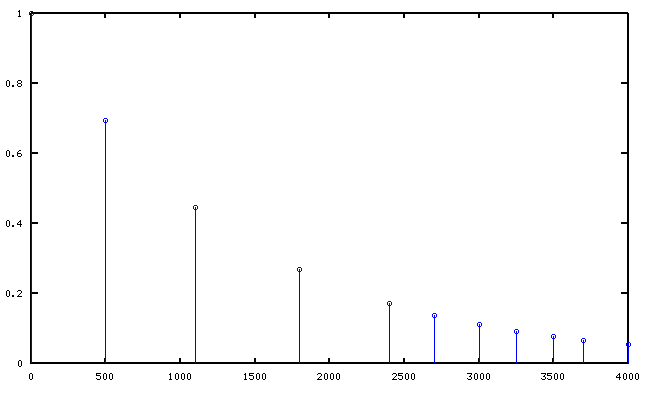
\includegraphics[scale=0.5]{Bilder/signalabgriffe.png}
	\caption{Raumimpulsantwort}
	\label{labelname}
\end{figure}

\subsubsection{Quellcode}
An diese STelle füge ich noch eine Quellcode umgebung ein
Hier ist meine neue Zeile zum mergetest im Kapitel 5\_0\_4

%ich muss dann oben noch \uspackage{listings} einfügen
%\usepackage{listings}

%\lstset{language=<Sprache>}
%\begin{slisting}[<Optionen>]
%	 quellcode hier einfügen
%\end{lstlisting}



\section{Schluss}
AAAAAAAAAAAAAAAAAAAAAAAAAAAchtung, wir testen den merge!


Dolore te feugait nulla facilisi nam liber tempor cum soluta nobis eleifend option. Amet consectetuer adipiscing elit sed diam nonummy nibh euismod tincidunt ut laoreet. In iis qui facit eorum; claritatem Investigationes demonstraverunt lectores legere me. In vulputate velit esse molestie consequat vel illum dolore. Wisi enim ad minim, veniam quis nostrud exerci. Facer possim assum typi non habent claritatem insitam est usus legentis lius quod.

Dolore te feugait nulla facilisi nam liber tempor cum soluta nobis eleifend option. Amet consectetuer adipiscing elit sed diam nonummy nibh euismod tincidunt ut laoreet. In iis qui facit eorum; claritatem Investigationes demonstraverunt lectores legere me. In vulputate velit esse molestie consequat vel illum dolore. Wisi enim ad minim, veniam quis nostrud exerci. Facer possim assum typi non habent claritatem insitam est usus legentis lius quod.

Dolore te feugait nulla facilisi nam liber tempor cum soluta nobis eleifend option. Amet consectetuer adipiscing elit sed diam nonummy nibh euismod tincidunt ut laoreet. In iis qui facit eorum; claritatem Investigationes demonstraverunt lectores legere me. In vulputate velit esse molestie consequat vel illum dolore. Wisi enim ad minim, veniam quis nostrud exerci. Facer possim assum typi non habent claritatem insitam est usus legentis lius quod.

Dolore te feugait nulla facilisi nam liber tempor cum soluta nobis eleifend option. Amet consectetuer adipiscing elit sed diam nonummy nibh euismod tincidunt ut laoreet. In iis qui facit eorum; claritatem Investigationes demonstraverunt lectores legere me. In vulputate velit esse molestie consequat vel illum dolore. Wisi enim ad minim, veniam quis nostrud exerci. Facer possim assum typi non habent claritatem insitam est usus legentis lius quod.

%Beginn einer neuen Seite
\clearpage

\section{Literaturverzeichnis}

lsf.uni-rostock.de, Veranstaltungsnummer 24141, Vorlesung Signalprozessortechnik, SS 2012
\newline

Versuchsanleitung Nr. 2 "`Digitale Filter"', Praktikum zur Veranstaltung "`Digitale Signalverarbeitung"' Institut für Nachrichtentechnik, Universität Rostock




\end{document}
%-------------------
%Hier endet der Text deiner Hausarbeit
%-------------------
%
%
%
%Ein längeres Zitat
%\begin{quote}
%Vel eum iriure dolor in hendrerit in vulputate velit esse. Modo typi qui nunc nobis, videntur %sollemnes in\footnote{fußnoten text}.
%\end{quote}